\chapter{Introducción}
\label{cap:capitulo1}
\setcounter{page}{1}

\begin{flushright}
\begin{minipage}[]{10cm}
\emph{Da el primer paso con fe, no tienes que ver todas las escaleras, sólo da el primer paso.}\\
\end{minipage}\\

Martin Luther King\\
\end{flushright}

\vspace{1cm}

Desde sus inicios, la robótica ha proporcionado un sinfin de posibilidades y alternativas ante problemas que anteriormente carecían de las soluciones adecuadas, pero, ¿qué es realmente la robótica?\\

Se podría definir \textit{robótica} como el proceso mediante el cual una máquina intercambia energía e información con su entorno, con el propósito de alcanzar una serie de objetivos específicos. Este campo tecnológico en expansión es el resultado de décadas de colaboración contínua entre biólogos, informáticos e ingenieros \cite{Koditschek21}.

Dada esta multidisciplina, la robótica abarca una amplia gama de aplicaciones, desde la industria hasta la medicina, pasando por la exploración espacial, la domótica o la conducción autónoma, entre otras. Es un campo en constante evolución, impulsado por la búsqueda de soluciones innovadoras para mejorar la calidad de vida y permitir superar desafíos de manera más eficiente y segura.\\

La industria agrícola no es una excepción, ya que ha contemplado históricamente tareas que requieren una dedicación laboral considerable. No obstante, gracias a la robótica y a los sistemas de visión artificial, surge la oportunidad de transformar una serie de procesos, como puede ser la recolección de cultivos, a través de la detección automatizada para su posterior recolección.\\

En las siguientes secciones describiremos brevemente algunas de las aplicaciones más importantes de la robótica en la sociedad actual, así como los distintos conceptos en los cuales se basa la investigación y el desarrollo llevado a cabo.\\

\section{Robots y robótica}
\label{sec:robótica} % etiqueta para luego referenciar esta sección

Según la Federación Internacional de Robots (IFR) se define robot según el vocabulario establecido por la International Organization for Standardization (ISO), y esto es como \textit{"mecanismo accionado programado con cierto grado de autonomía para realizar tareas de locomoción, manipulación o posicionamiento"} \cite{ISO8373}.\\  

El término \textit{“robot”} fue utilizado por primera vez por Karel Capek (en su obra de teatro “Rossum’s Universal Robots” publicada en 1920. Esta palabra viene del vocablo checo \textit{“robota”} que significa “trabajo”, en el sentido de la obligatoriedad, entendido como servidumbre, trabajo forzado o esclavitud \cite{Sanchez07a}.

Aunque esta definición es un punto de partida, es cierto que es posible diferir en aspectos como si un robot debe controlarse automáticamente o podría ser autónomo o si un robot debe ser reprogramable. A un nivel más amplio, cualquier máquina que pueda utilizarse para llevar a cabo acciones o tareas complejas de forma automática puede considerarse un robot \cite{Raj19}.\\

Históricamente, las civilizaciones antiguas, como la egipcia y la griega, dieron los primeros pasos en lo que se puede denominar \textit{robótica clásica}, construyendo autómatas y mecanismos diseñados para imitar acciones humanas, con características mecánicas rudimentarias. 
Con el paso del tiempo, la ciencia y la ingeniería avanzaron, y los conceptos de la robótica comenzaron a tomar forma más definida hasta que, en el siglo XX, con el desarrollo de la ingeniería en sus diferentes ramas (mecánica, electrónica, informática, telecomunicaciones), \textbf{\emph{Isaac Asimov}} (1920-1992) utilizó por primera vez el término \textit{“robótica”} y postuló las tres leyes de la robótica en su libro \textit{I Robot} publicado en 1950, coincidiendo con el apogeo de la \textit{robótica moderna} \cite{Sanchez07b}.\\


\begin{table} [h!]
  \begin{center}
    \begin{tabular}{p{15cm}} % Ajustar el ancho según necesidades
      \hline
      1. Un robot no debe dañar a un ser humano ni, por su pasividad, dejar que un ser humano sufra daño.\\\\
    
      2. Un robot no debe obedecer las órdenes que le son dadas por un ser humano, excepto cuando estas órdenes están en oposición con la primera Ley.\\\\
    
      3. Un robot debe proteger su propia existencia, hasta donde esta protección no esté en conflicto con la primera o segunda Ley. \\
      \hline
    \end{tabular}
  \end{center}
  \caption{Las tres leyes de la robótica según Asimov.}
  \label{cuadro:leyesrobotica_Asimov}
\end{table}

Asimov consideró necesario añadir una cuarta ley, antepuesta a las demás, la número cero, que afirma que un robot no debe actuar simplemente para satisfacer intereses individuales, sino que sus acciones deben preservar el beneficio común de toda la humanidad \cite{Sanchez07b}.\\\\

Es también en 1950, cuando \textbf{\emph{Alan Mathison Turing}} publica \textit{“Computing Machinery and Intelligence”} y propone una prueba (test o máquina de Touring), en forma de entidad matemática abstracta, que demuestra la existencia de problemas computacionales irresolubles que ninguna máquina es capaz de solventar. Se puede afirmar que un programa de ordenador no llegará nunca a ser tan inteligente como un ser humano y que un robot no podrá suplir al ser humano de forma completa, \cite{Sanchez07b} preocupación sobre el potencial de sustitución de la mano de obra, que históricamente, ha atenuado el entusiasmo en torno a las nuevas tecnologías \cite{Mokyr15}. 

\begin{figure} [h!]
  \begin{center}
    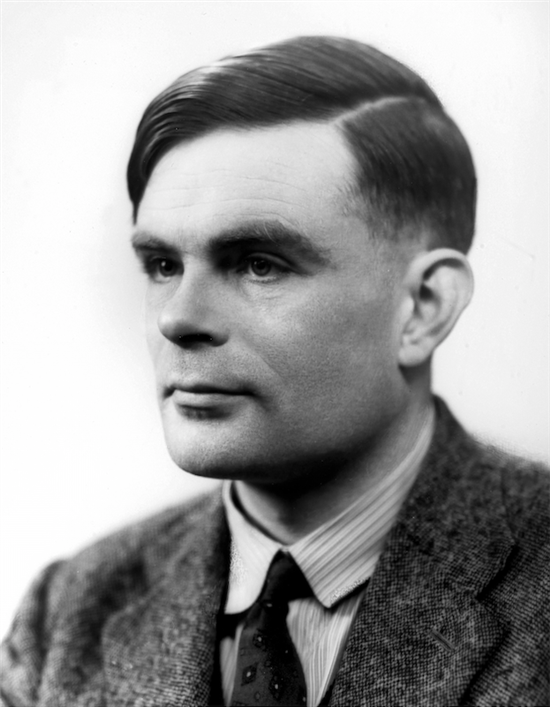
\includegraphics[width=8cm]{figs/Alan_Turing.jpg}
  \end{center}
  \caption{El matemático Alan Turing.}
  \label{fig:alanturing}
\end{figure}


A partir de todos estos avances y del interés por automatizar las tareas de producción, la robótica va adquiriendo un gran desarrollo \cite{Sanchez07b}. Es debido a este desarrollo, que atendiendo al propósito y al contexto en el que se utilicen estos robots, se fueron creando varios grupos en función de los que clasificarles. Estos tres grandes grupos en función de una serie de criterios generales fueron: \textit{robots industriales}, \textit{robots de servicio} y \textit{robots médicos}.\\

\subsection{Robot Industrial}
\label{sec:robot_industrial}

Se define \textit{robot industrial} como un "manipulador polivalente, reprogramable y controlado automáticamente, programable en tres o más ejes, que puede ser fijo o móvil para su uso en aplicaciones de automatización industrial" \cite{ISO8373}.



\subsection{Robot de Servicio}
\label{sec:robot_servicio}

Se define \textit{robot de servicio} como un robot que realiza tareas útiles para las personas o los equipos, incluyendo en esta la manipulación o el servicio de artículos, el transporte, el apoyo físico, la orientación o información, el aseo personal, la cocina y la manipulación de alimentos y la limpieza en el ámbito personal, y la inspección, vigilancia, manipulación de objetos, transporte de personas, orientación o información, cocina y manipulación de alimentos y limpieza en el ámbito profesional \cite{ISO8373}.
 

\subsection{Robot Médico}
\label{sec:robotica_industrial} 

Se define \textit{robot médico} a aquellos dispositivos electromecánicos que desempeñan parcial o totalmente algunas funciones de los seres humanos o de sus órganos al resolver problemas médicos, ayudando a mejorar la asistencia al paciente y los resultados, a la vez que aumenta la eficiencia operativa \cite{Kraevsky10}.\\

En los textos puedes poner palabras en \textit{cursiva}, para aquellas expresiones en sentido \textit{figurado}, palabras como \textit{robota}, que está fuera del diccionario castellano, o bien para resaltar palabras de una colección: \textit{(a)} es la primera letra del abecedario, \textit{(b)} es la segunda, etc.\\

Al poner las dos líneas del anterior párrafo, este aparecerá separado del anterior. Si no las pongo, los párrafos aparecerán pegados. Sigue el criterio que consideres más oportuno.

\section{Segunda sección}
\label{sec:segundaseccion}

No olvides incluir imágenes y referenciarlas, como la Figura \ref{fig:roomba}.

\begin{figure} [h!]
  \begin{center}
    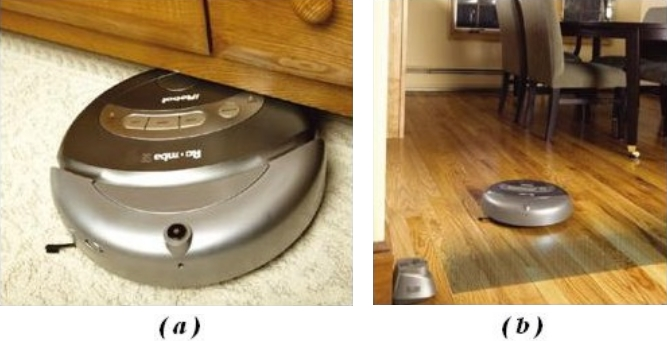
\includegraphics[width=8cm]{figs/roomba}
  \end{center}
  \caption{Robot aspirador Roomba de iRobot.}
  \label{fig:roomba}
\end{figure}\

Ni tampoco olvides de poner las URLs como notas al pie. Por ejemplo, si hablo de la Robocup\footnote{\url{http://www.robocup.org}}.

\subsection{Números}
\label{sec:subseccion}

En lugar de tener secciones interminables, como la Sección \ref{sec:miseccion}, divídelas en subsecciones.

Para hablar de números, mételos en el entorno \textit{math} de \LaTeX, por ejemplo, $1.5Kg$. También puedes usar el símbolo del Euro como aquí: 1.500\euro.

\subsection{Listas}

Cuando describas una colección, usa \texttt{itemize} para ítems o \texttt{enumerate} para enumerados. Por ejemplo:

\begin{itemize}
 \item \textit{Entorno de simulación.} Hemos usado dos entornos de simulación: uno en 3D y otro en 2D.
 \item \textit{Entornos reales.} Dentro del campus, hemos realizado experimentos en Biblioteca y en el edificio de Gestión.
\end{itemize}\

\begin{enumerate}
 \item Primer elemento de la colección.
 \item Segundo elemento de la colección.
\end{enumerate}\

\paragraph{Referencias bibliográficas}
\label{sec:referencias}

% Cita, sobre todo en este capítulo, referencias bibliográficas que respalden tu argumento. Para citarlas basta con poner la instrucción \verb|\cite| con el identificador de la cita. Por ejemplo: libros como \cite{vega12e}, artículos como \cite{vega19b}, URLs como \cite{vega19a}, tesis como \cite{vega18b}, congresos como \cite{vega18a}, u otros trabajos fin de grado como \cite{vega08b}.

Las referencias, con todo su contenido, están recogidas en el fichero \texttt{bibliografia.bib}. El contenido de estas referencias está en formato \texttt{BibTex}. Este formato se puede obtener en muchas ocasiones directamente, desde plataformas como \texttt{Google Scholar} u otros repositorios de recursos científicos.

Existen numerosos estilos para reflejar una referencia bibliográfica. El estilo establecido por defecto en este documento es APA, que es uno de los estilos más comunes, pero lo puedes modificar en el archivo \texttt{memoria.tex}; concretamente, cambiando el campo \verb|apalike| a otro en la instrucción \verb|\bibliographystyle{apalike}|. 

\

\

\

Y, para terminar este capítulo, resume brevemente qué vas a contar en los siguientes.
